\documentclass{standalone}
\usepackage{tikz}
\usepackage{color}
\usetikzlibrary{positioning, shapes, arrows.meta, calc, decorations.pathreplacing}

\definecolor{myblue}{RGB}{82,126,171}
\definecolor{myred}{RGB}{168, 50, 50}

\tikzset{
  square/.style={draw,outer sep=5,inner sep=3,minimum size=10,line width=0, 
    very thick, draw=myblue, top color=white,bottom color=white},
  noborder/.style={draw,outer sep=0,inner sep=0,minimum size=20,line width=1, 
    draw=none, scale=1, anchor=west},
  blue/.style={draw,outer sep=35,inner sep=3,minimum size=20, line width=1, 
    very thick, draw=none, top color=myblue, bottom color=myblue, scale=1.25},
   noborderr/.style={draw,outer sep=0,inner sep=0,minimum size=20,line width=1, 
    draw=none, scale=1, anchor=west}
}

\begin{document}

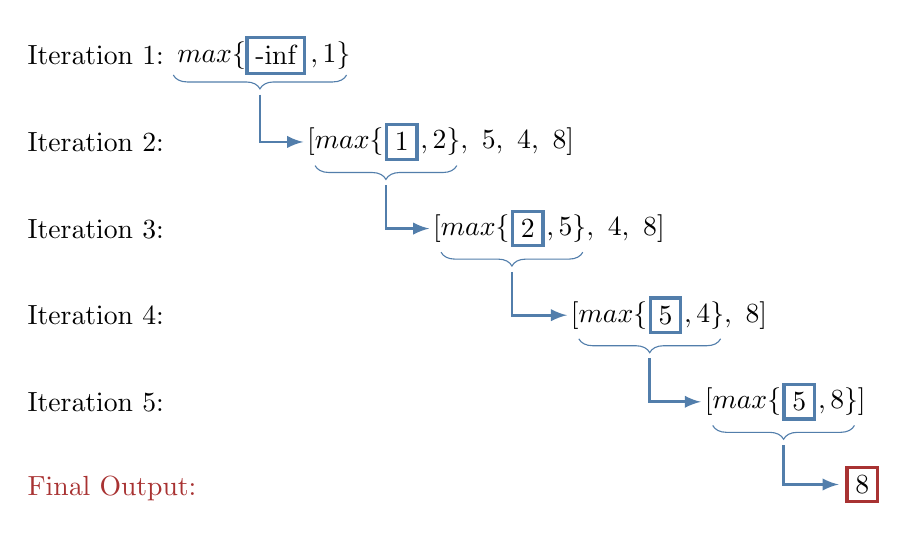
\begin{tikzpicture}



\draw[decorate,color=myblue,decoration={brace,amplitude=5pt}] (-0.2,2.55) -- (-2.4,2.55);
\draw[-latex,line width=1 pt,color=myblue] (-1.3,2.3) |- (-0.75,1.7);

\node [noborderr] at (-2.35,2.8) {$max\{~~~~~~~,1\}$};
\node [square] at (-1.1,2.8) {-inf};

\draw[decorate,color=myblue,decoration={brace,amplitude=5pt}] (1.2,1.4) -- (-0.6,1.4);
\draw[-latex,line width=1 pt,color=myblue] (0.3,1.15) |- (0.85,0.6);

\node [noborderr] at (-0.7,1.7) {$[max\{~~~~,2\}, ~5, ~4, ~8]$};
\node [square] at (0.5,1.7) {$1$};

\draw[decorate,color=myblue,decoration={brace,amplitude=5pt}] (2.8,0.3) -- (1,0.3);
\draw[-latex,line width=1 pt, color=myblue] (1.9,0.05) |- (2.6,-0.5);

\node [noborderr] at (0.9,0.6) {$[max\{~~~~,5\},  ~4, ~8]$};
\node [square] at (2.1,0.6) {$2$};


\draw[decorate,color=myblue,decoration={brace,amplitude=5pt}] (4.55,-0.8) -- (2.75,-0.8);
\draw[-latex,line width=1 pt,color=myblue] (3.65,-1.05) |- (4.3,-1.6);

\node [noborderr] at (2.65,-0.5) {$[max\{~~~~,4\},  ~8]$};
\node [square] at (3.85,-0.5) {$5$};


\draw[decorate,color=myblue,decoration={brace,amplitude=5pt}] (6.25,-1.9) -- (4.45,-1.9);
\draw[-latex, line width=1 pt, color=myblue] (5.35,-2.15) |- (6.05,-2.65);

\node [noborderr] at (4.35,-1.6) {$[max\{~~~~,8\}]$};
\node [square] at (5.55,-1.6) {$5$};
\node [square,draw=myred] at (6.35,-2.65) {$8$};

\node [noborderr] at (-4.25,2.8) {Iteration 1:};
\node [noborderr] at (-4.25,1.7) {Iteration 2:};
\node [noborderr] at (-4.25,0.6) {Iteration 3:};
\node [noborderr] at (-4.25,-0.5) {Iteration 4:};
\node [noborderr] at (-4.25,-1.6) {Iteration 5:};
\node [noborderr, color=myred] at (-4.25,-2.7) {Final Output:};


\end{tikzpicture}

\end{document}
